\chapter{Lexical analysis}
\lecture{4}{4/2}

Lexical analysis is the first stage in compilation.
It reads a character stream and produces \emph{tokens}.

We separate lexical and syntax analysis as
\begin{enumerate}
    \item it gives simplicity in design;
    \item we can have improved efficiency; and
    \item modularity means portability.
\end{enumerate}

\begin{definition}[Token]
    A \textbf{token} is a notation representing a \emph{lexical unit}
    consisting of a \emph{token name} and an (optional) \emph{attribute value}.
\end{definition}

Tokens are the input to our parser (the next stage of compilation).

\begin{definition}[Lexeme]
    A \textbf{lexeme} is a sequence of characters that \emph{matches} a token.
\end{definition}

\begin{example}
    Lets look at some lexemes and their corresponding tokens.
    \begin{center}
        \ttfamily
        \begin{tabular}{ll}
            \toprule
            \normalfont Token & \normalfont Lexeme \\ 
            \midrule
            if & if \\
            else & else \\
            comparison & >, >=. == \\
            number & 3, 10.2 \\
            literal & 'any string', 'hi' \\
            \bottomrule
        \end{tabular}
    \end{center}
\end{example}

In some cases, many lexemes match a given token.
So the compiler must provide additional information to identify the lexeme,
this is our \emph{attribute values} mentioned earlier.

Token names influence \emph{parsing decisions} while
attribute values influence \emph{translation decisions}.

Attributes can correspond to multiple pieces of information, such as
\begin{enumerate}
    \item its lexeme;
    \item type; and
    \item line number in source code.
\end{enumerate}
All of this information is stored in the \emph{symbol table}.

Some tokens are \emph{reserved} and take no attribute,
such as \texttt{if}, \texttt{for}, etc.

We can express patterns of tokens as \emph{regular expressions}
defined by \emph{regular definitions}.
Syntax can be expressed by \emph{context-free grammars} (CFG).

\begin{example}[CFG for branching]
    \hfill
    \begin{center}
        \ttfamily
        \begin{tabular}{lll}
            \toprule
            stmt & $\to$ & \textbf{if} expr \textbf{then} stmt \\
                 &       & \textbf{if} expr \textbf{then} stmt \textbf{else} stmt \\
                 &       & $\varepsilon$ \\
            expr & $\to$ & term \textbf{relop} term \\
                 &       & term \\
            term & $\to$ & \textbf{id} \\
                 &       & \textbf{number} \\
            \bottomrule
        \end{tabular}
    \end{center}
    All bolded words are terminal.
    Note that \texttt{relop} is a comparison operator.
\end{example}

\begin{example}[RE for tokens]
    \hfill
    \begin{center}
        \ttfamily
        \begin{tabular}{lll}
            \toprule
            \textbf{if}     & $\to$ & if                         \\
            \textbf{then}   & $\to$ & then                       \\
            \textbf{else}   & $\to$ & else                       \\
            \textbf{id}     & $\to$ & letter(letter$\mid$digit)* \\
            \textbf{letter} & $\to$ & [a-zA-Z]                   \\
            \textbf{digit}  & $\to$ & [0-9]                      \\
            \textbf{number} & $\to$ & digit+(digit+)?            \\
            \bottomrule
        \end{tabular}
    \end{center}
    Here \texttt{+} means one or more and \texttt{?} means optional.
\end{example}

\begin{example}[Summary table]
    \hfill
    \begin{center}
        \ttfamily
        \begin{tabular}{lll}
            \toprule
            \normalfont Lexemes & \normalfont Token name & \normalfont Attribute \\
            \midrule
            if      & if    & -       \\
            then    & then  & -       \\
            any id  & id    & pointer \\
            any num & num   & pointer \\
            <       & relop & LT      \\
            >       & relop & GT      \\
            ==      & relop & EQ      \\
            <>      & relop & NE      \\
            <=      & relop & LE      \\
            >=      & relop & GE      \\
            \bottomrule
        \end{tabular}
    \end{center}
\end{example}

\begin{remark}
    Whitespace is ignored in lexical analysis (do \emph{not} see Python).
\end{remark}

When we are looking for lexemes, we have a pointer at the start
and another scanning forward until we find a pattern.
Patterns can be recognised by a DFA and modelled with a transition diagram,
as shown below (\texttt{o} means other).

\begin{center}
    \ttfamily
    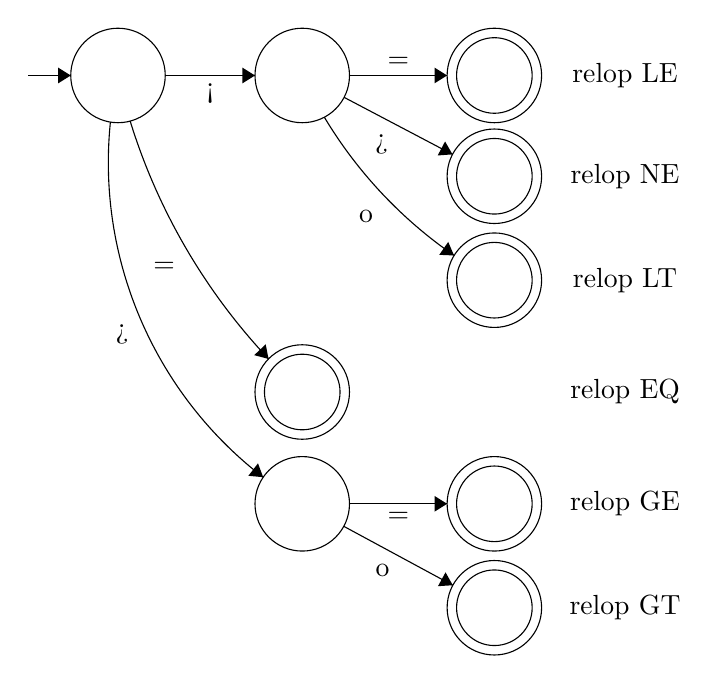
\begin{tikzpicture}[scale=0.2]
        \tikzstyle{every node}+=[inner sep=0pt]
        \draw [black] (10.9,-7) circle (3);
        \draw [black] (22.6,-7) circle (3);
        \draw [black] (34.8,-7) circle (3);
        \draw [black] (34.8,-7) circle (2.4);
        \draw [black] (34.8,-13.4) circle (3);
        \draw [black] (34.8,-13.4) circle (2.4);
        \draw [black] (34.8,-20) circle (3);
        \draw [black] (34.8,-20) circle (2.4);
        \draw [black] (22.6,-34.2) circle (3);
        \draw [black] (34.8,-34.2) circle (3);
        \draw [black] (34.8,-34.2) circle (2.4);
        \draw [black] (34.8,-40.8) circle (3);
        \draw [black] (34.8,-40.8) circle (2.4);
        \draw [black] (22.6,-27.1) circle (3);
        \draw [black] (22.6,-27.1) circle (2.4);
        \draw (43.1,-7) node {relop LE};
        \draw (43.1,-13.4) node {relop NE};
        \draw (43.1,-20) node {relop LT};
        \draw (43.1,-34.2) node {relop GE};
        \draw (43.1,-40.8) node {relop GT};
        \draw (43.1,-27.1) node {relop EQ};
        \draw [black] (5.2,-7) -- (7.9,-7);
        \fill [black] (7.9,-7) -- (7.1,-6.5) -- (7.1,-7.5);
        \draw [black] (13.9,-7) -- (19.6,-7);
        \fill [black] (19.6,-7) -- (18.8,-6.5) -- (18.8,-7.5);
        \draw (16.75,-7.5) node [below] {<};
        \draw [black] (25.6,-7) -- (31.8,-7);
        \fill [black] (31.8,-7) -- (31,-6.5) -- (31,-7.5);
        \draw (28.7,-6.5) node [above] {=};
        \draw [black] (25.26,-8.39) -- (32.14,-12.01);
        \fill [black] (32.14,-12.01) -- (31.67,-11.19) -- (31.2,-12.08);
        \draw (27.64,-10.7) node [below] {>};
        \draw [black] (32.245,-18.431) arc (-124.57497:-149.06163:28.394);
        \fill [black] (32.24,-18.43) -- (31.87,-17.57) -- (31.3,-18.39);
        \draw (27.12,-15.95) node [left] {o};
        \draw [black] (20.462,-24.996) arc (-136.75631:-162.83722:38.713);
        \fill [black] (20.46,-25) -- (20.28,-24.07) -- (19.55,-24.76);
        \draw (14.55,-19.19) node [left] {=};
        \draw [black] (20.12,-32.515) arc (-127.60731:-185.84306:25.229);
        \fill [black] (20.12,-32.51) -- (19.79,-31.63) -- (19.18,-32.42);
        \draw (11.61,-23.46) node [left] {>};
        \draw [black] (25.6,-34.2) -- (31.8,-34.2);
        \fill [black] (31.8,-34.2) -- (31,-33.7) -- (31,-34.7);
        \draw (28.7,-34.7) node [below] {=};
        \draw [black] (25.24,-35.63) -- (32.16,-39.37);
        \fill [black] (32.16,-39.37) -- (31.7,-38.55) -- (31.22,-39.43);
        \draw (27.7,-38) node [below] {o};
    \end{tikzpicture}
\end{center}

\begin{example}
    Consider the following DFA.
    \begin{center}
        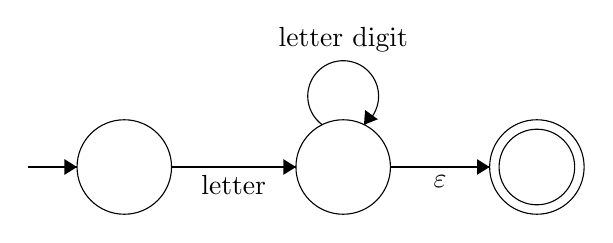
\begin{tikzpicture}[scale=0.2]
            \tikzstyle{every node}+=[inner sep=0pt]
            \draw [black] (11.6,-15.9) circle (3);
            \draw [black] (25.5,-15.9) circle (3);
            \draw [black] (37.8,-15.9) circle (3);
            \draw [black] (37.8,-15.9) circle (2.4);
            \draw [black] (5.5,-15.9) -- (8.6,-15.9);
            \fill [black] (8.6,-15.9) -- (7.8,-15.4) -- (7.8,-16.4);
            \draw [black] (14.6,-15.9) -- (22.5,-15.9);
            \fill [black] (22.5,-15.9) -- (21.7,-15.4) -- (21.7,-16.4);
            \draw (18.55,-16.4) node [below] {letter};
            \draw [black] (28.5,-15.9) -- (34.8,-15.9);
            \fill [black] (34.8,-15.9) -- (34,-15.4) -- (34,-16.4);
            \draw (31.65,-16.4) node [below] {$\varepsilon$};
            \draw [black] (24.177,-13.22) arc (234:-54:2.25);
            \draw (25.5,-8.65) node [above] {letter digit};
            \fill [black] (26.82,-13.22) -- (27.7,-12.87) -- (26.89,-12.28);
        \end{tikzpicture}
    \end{center}
    This DFA will also accept \emph{reserved words}.
    We can handle this in two ways:
    \begin{enumerate}
        \item install reserved words into the symbol table; or
        \item create separate transition diagarms for reserved words, as below.
    \end{enumerate}
    \begin{center}
        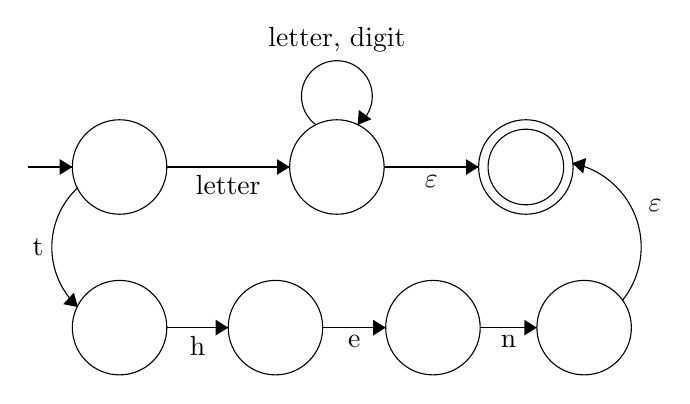
\begin{tikzpicture}[scale=0.2]
            \tikzstyle{every node}+=[inner sep=0pt]
            \draw [black] (10.4,-15.9) circle (3);
            \draw [black] (24.2,-15.9) circle (3);
            \draw [black] (36.2,-15.9) circle (3);
            \draw [black] (36.2,-15.9) circle (2.4);
            \draw [black] (10.4,-26.1) circle (3);
            \draw [black] (20.3,-26.1) circle (3);
            \draw [black] (30.3,-26.1) circle (3);
            \draw [black] (39.9,-26.1) circle (3);
            \draw [black] (4.6,-15.9) -- (7.4,-15.9);
            \fill [black] (7.4,-15.9) -- (6.6,-15.4) -- (6.6,-16.4);
            \draw [black] (22.877,-13.22) arc (234:-54:2.25);
            \draw (24.2,-8.65) node [above] {letter, digit};
            \fill [black] (25.52,-13.22) -- (26.4,-12.87) -- (25.59,-12.28);
            \draw [black] (13.4,-15.9) -- (21.2,-15.9);
            \fill [black] (21.2,-15.9) -- (20.4,-15.4) -- (20.4,-16.4);
            \draw (17.3,-16.4) node [below] {letter};
            \draw [black] (27.2,-15.9) -- (33.2,-15.9);
            \fill [black] (33.2,-15.9) -- (32.4,-15.4) -- (32.4,-16.4);
            \draw (30.2,-16.4) node [below] {$\varepsilon$};
            \draw [black] (7.748,-24.789) arc (-132.91218:-227.08782:5.174);
            \fill [black] (7.75,-24.79) -- (7.5,-23.88) -- (6.82,-24.61);
            \draw (5.6,-21) node [left] {t};
            \draw [black] (13.4,-26.1) -- (17.3,-26.1);
            \fill [black] (17.3,-26.1) -- (16.5,-25.6) -- (16.5,-26.6);
            \draw (15.35,-26.6) node [below] {h};
            \draw [black] (23.3,-26.1) -- (27.3,-26.1);
            \fill [black] (27.3,-26.1) -- (26.5,-25.6) -- (26.5,-26.6);
            \draw (25.3,-26.6) node [below] {e};
            \draw [black] (33.3,-26.1) -- (36.9,-26.1);
            \fill [black] (36.9,-26.1) -- (36.1,-25.6) -- (36.1,-26.6);
            \draw (35.1,-26.6) node [below] {n};
            \draw [black] (39.152,-15.662) arc (78.77468:-38.89869:5.425);
            \fill [black] (39.15,-15.66) -- (39.84,-16.31) -- (40.03,-15.33);
            \draw (43.96,-18.35) node [right] {$\varepsilon$};
        \end{tikzpicture}
    \end{center}
    Creating separate transition diagrams reduces the load on the symbol table; 
    however, adds a lot of computation for every lexeme processed.
\end{example}
